% !TeX program = xelatex
\documentclass[a4paper,10pt]{article}

% ============================================================================
% ១. កញ្ចប់បណ្ណាល័យ និងការកំណត់ទំព័រ (Packages & Page Setup — តាមគំរូ ls_plan.tex)
% ============================================================================
\usepackage[a4paper, left=0.95cm, right=0.95cm, top=0.85cm, bottom=0.92cm, footskip=0.52cm]{geometry}
\usepackage{amsmath}
\usepackage{unicode-math}
\usepackage{fontspec}
\usepackage{longtable, array, multirow, colortbl}
\usepackage[table]{xcolor}
\usepackage{enumitem}
\usepackage{pifont}
\usepackage{fancyhdr}
\usepackage{tikz}
\usetikzlibrary{calc, arrows.meta, decorations.pathreplacing, patterns, positioning, babel}

\makeatletter
\let\@expl@@@mark@update@singlecol@structures@@\relax
\makeatother

% --- ប្រព័ន្ធស្វែងរកទីតាំងពុម្ពអក្សរស្វ័យប្រវត្តិ (Windows Local + Cloud Repo fonts/) ---
\providecommand{\NGSFindFonts}{%
  \IfFileExists{C:/Windows/Fonts/cambria.ttc}{%
    \def\NGSSysPath{C:/Windows/Fonts/}%
    \def\NGSUserPath{C:/Users/KIT/AppData/Local/Microsoft/Windows/Fonts/}%
  }{%
    \IfFileExists{./fonts/KhmerOSsiemreap.ttf}{\def\NGSSysPath{./fonts/}\def\NGSUserPath{./fonts/}}{%
    \IfFileExists{../fonts/KhmerOSsiemreap.ttf}{\def\NGSSysPath{../fonts/}\def\NGSUserPath{../fonts/}}{%
    \IfFileExists{../../fonts/KhmerOSsiemreap.ttf}{\def\NGSSysPath{../../fonts/}\def\NGSUserPath{../../fonts/}}{%
    \IfFileExists{../../../fonts/KhmerOSsiemreap.ttf}{\def\NGSSysPath{../../../fonts/}\def\NGSUserPath{../../../fonts/}}{%
    \IfFileExists{../../../../fonts/KhmerOSsiemreap.ttf}{\def\NGSSysPath{../../../../fonts/}\def\NGSUserPath{../../../../fonts/}}{%
    \IfFileExists{../../../../../fonts/KhmerOSsiemreap.ttf}{\def\NGSSysPath{../../../../../fonts/}\def\NGSUserPath{../../../../../fonts/}}{%
    \IfFileExists{../../../../../../fonts/KhmerOSsiemreap.ttf}{\def\NGSSysPath{../../../../../../fonts/}\def\NGSUserPath{../../../../../../fonts/}}{%
      \def\NGSSysPath{../../../../../../../fonts/}\def\NGSUserPath{../../../../../../../fonts/}%
    }}}}}}}%
  }%
}
\NGSFindFonts

% ============================================================================
% ២. កំណត់ពុម្ពអក្សរ (Fonts — តាមគំរូ ls_plan.tex)
% ============================================================================
\setmathfont[Path={\NGSSysPath}, FontIndex=1, Scale=1.02]{cambria.ttc}
\defaultfontfeatures{Ligatures=TeX}

\setmainfont[
  Path={\NGSUserPath},
  Extension=.ttf,
  Script=Khmer,
  BoldFont={KhmerOSsiemreap},
  BoldFeatures={FakeBold=1.8},
  ItalicFont={KhmerOSsiemreap},
  ItalicFeatures={FakeSlant=0.25},
  BoldItalicFont={KhmerOSsiemreap},
  BoldItalicFeatures={FakeBold=1.8, FakeSlant=0.25}
]{KhmerOSsiemreap}

\newfontfamily\muol[Path={\NGSUserPath}, Extension=.ttf, Script=Khmer]{KhmerOSmuollight}
\newfontfamily\Tacteing[Path={\NGSUserPath}, Extension=.TTF]{TACTENG}
\newfontfamily\TimesEn[Path={\NGSSysPath}, Extension=.ttf, BoldFont={timesbd}, ItalicFont={timesi}, BoldItalicFont={timesbi}]{times}
\newfontfamily\CalibriFont[Path={\NGSSysPath}, Extension=.ttf]{calibri}
\newfontfamily\CourierCirc[Path={\NGSSysPath}, Extension=.ttf]{cour}

\XeTeXlinebreaklocale "km"
\XeTeXlinebreakskip = 0pt plus 1pt minus 0.1pt

% ============================================================================
% ៣. ពណ៌ និងការតុបតែង (Colors & Styles)
% ============================================================================
\definecolor{stepbg}{HTML}{D9D9D9}
\definecolor{headgray}{HTML}{E6E6E6}
\definecolor{emphred}{HTML}{C00000}

\pagestyle{fancy}
\fancyhf{}
\renewcommand{\headrulewidth}{0pt}
\fancyfoot[R]{\CalibriFont\fontsize{9pt}{11pt}\selectfont\thepage}

\setlength{\parindent}{0pt}
\setlength{\parskip}{0pt}
\setlength{\tabcolsep}{4.5pt}
\setlength{\LTpre}{2pt}
\setlength{\LTpost}{2pt}

\newcolumntype{L}[1]{>{\raggedright\arraybackslash}p{#1}}
\newcolumntype{C}[1]{>{\centering\arraybackslash}p{#1}}

% ============================================================================
% ៤. ពាក្យបញ្ជាជំនួយ (Helper Macros)
% ============================================================================
\newcommand{\en}[1]{{\TimesEn #1}}
\newcommand{\enbf}[1]{{\TimesEn\bfseries #1}}
\newcommand{\khmflourish}{{\Tacteing\fontsize{15pt}{15pt}\selectfont 3}}
\newcommand{\wcirc}{{\CourierCirc\fontsize{9.5pt}{11pt}\selectfont o}}
\newcommand{\ditem}{{\fontsize{7.5pt}{10pt}\selectfont\ding{117}}\ }
\newcommand{\fiveE}[1]{\textcolor{emphred}{\CalibriFont\bfseries #1}}
\newcommand{\redsub}[1]{\textcolor{emphred}{#1}}
\newcommand{\timenote}[1]{\textcolor{emphred}{\textit{#1}}}
\newcommand{\stepheader}[1]{\multicolumn{3}{|c|}{\cellcolor{stepbg}\muol #1} \\ \hline}
\newcommand{\cfig}[1]{{\centering\vspace{3pt}#1\vspace{3pt}\par}}
\newcommand{\cnum}[1]{\mbox{\fontsize{10.5pt}{12pt}\selectfont\ding{\numexpr181+#1\relax}}}
\newcommand{\unit}[1]{\,\text{\en{#1}}}
\newcommand{\riel}{\,\text{៛}}
\newcommand{\graybox}[1]{\colorbox{headgray}{\strut #1}}

% ============================================================================
% ៥. រូបភាព TikZ ស-ខ្មៅ សម្រាប់បង្រៀនលើក្ដារខៀន និងសន្លឹកកិច្ចការ (B&W Diagrams)
% ============================================================================

% ១. E1 Engage: អន្ទាក់សម្រួលតែតួទី១ ពេលចែកពហុធានឹងឯកធា (ទំ.៦០)
\newcommand{\figEngageALGFiveFour}{%
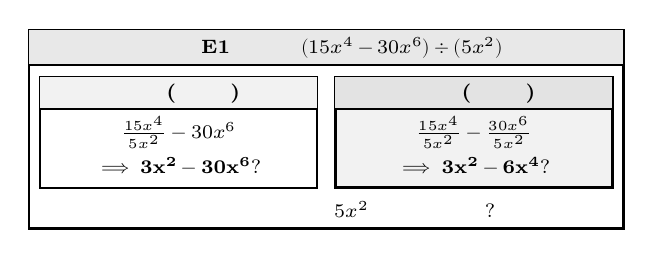
\begin{tikzpicture}[x=1cm, y=1cm, every node/.style={font=\scriptsize, text=black}]
  \draw[black, line width=0.9pt] (0,0) rectangle (7.55,2.52);
  \fill[gray!18] (0,2.08) rectangle (7.55,2.52);
  \draw[black, line width=0.6pt] (0,2.08) -- (7.55,2.08);
  \node at (3.775,2.30) {\textbf{បេសកកម្ម \en{E1}៖ គណនាផលចែក $(15x^4 - 30x^6) \div (5x^2)$}};

  % Student A
  \draw[black, line width=0.8pt] (0.14,0.52) rectangle (3.66,1.92);
  \fill[gray!10] (0.14,1.52) rectangle (3.66,1.92);
  \draw[black, line width=0.5pt] (0.14,1.52) -- (3.66,1.52);
  \node at (1.90,1.72) {\textbf{សិស្ស ក (ចែកតែតួទី១)}};
  \node at (1.90,1.22) {$\tfrac{15x^4}{5x^2} - 30x^6$};
  \node at (1.90,0.80) {$\implies \mathbf{3x^2 - 30x^6}$?};

  % Student B
  \draw[black, line width=0.95pt, fill=gray!10] (3.89,0.52) rectangle (7.41,1.92);
  \fill[gray!22] (3.89,1.52) rectangle (7.41,1.92);
  \draw[black, line width=0.55pt] (3.89,1.52) -- (7.41,1.52);
  \node at (5.65,1.72) {\textbf{សិស្ស ខ (ចែកគ្រប់តួ)}};
  \node at (5.65,1.22) {$\tfrac{15x^4}{5x^2} - \tfrac{30x^6}{5x^2}$};
  \node at (5.65,0.80) {$\implies \mathbf{3x^2 - 6x^4}$?};

  \node at (3.775,0.24) {\textbf{សំណួរគន្លឹះ៖} ពេលចែកពហុធានឹងឯកធា $5x^2$ តើត្រូវចែកប៉ុន្មានតួ?};
\end{tikzpicture}}

% ២. E2 Explore: គំរូផ្ទៃរូបថតប្រាសាទ (3x+2)(x+1) និងវិធីចែកជួរឈរ (ទំ.៥៩--៦១)
\newcommand{\figExploreALGFiveFour}{%
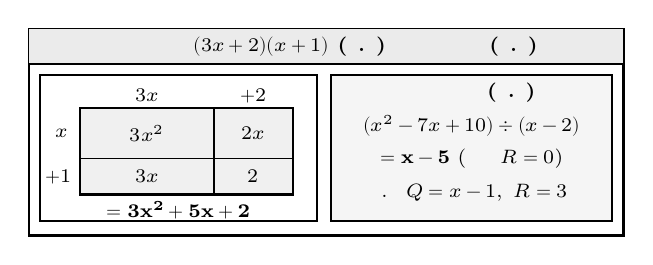
\begin{tikzpicture}[x=1cm, y=1cm, every node/.style={font=\scriptsize, text=black}]
  \draw[black, line width=0.9pt] (0,0) rectangle (7.55,2.62);
  \fill[gray!16] (0,2.18) rectangle (7.55,2.62);
  \draw[black, line width=0.6pt] (0,2.18) -- (7.55,2.18);
  \node at (3.775,2.40) {\textbf{គំរូផ្ទៃក្រឡា $(3x+2)(x+1)$ (ទំ.៥៩) និងចែកពហុធាជួរឈរ (ទំ.៦១)}};

  % Left: Area grid (3x+2)(x+1)
  \draw[black, line width=0.8pt] (0.14,0.18) rectangle (3.66,2.04);
  \draw[black, line width=0.85pt, fill=gray!12] (0.65,0.52) rectangle (3.35,1.62);
  \draw[black, line width=0.6pt] (2.35,0.52) -- (2.35,1.62);
  \draw[black, line width=0.6pt] (0.65,0.98) -- (3.35,0.98);
  \node at (1.50,1.78) {$3x$};
  \node at (2.85,1.78) {$+2$};
  \node at (0.42,1.30) {$x$};
  \node at (0.38,0.75) {$+1$};
  \node at (1.50,1.30) {$3x^2$};
  \node at (2.85,1.30) {$2x$};
  \node at (1.50,0.75) {$3x$};
  \node at (2.85,0.75) {$2$};
  \node at (1.90,0.32) {$= \mathbf{3x^2 + 5x + 2}$};

  % Right: Polynomial division (x^2 - 7x + 10) / (x - 2)
  \draw[black, line width=0.8pt, fill=gray!8] (3.84,0.18) rectangle (7.41,2.04);
  \node at (5.625,1.82) {\textbf{ចែកពហុធាជួរឈរ (ទំ.៦១)}};
  \node at (5.625,1.40) {$(x^2 - 7x + 10) \div (x - 2)$};
  \node at (5.625,0.98) {$= \mathbf{x - 5}$ (សំណល់ $R = 0$)};
  \node at (5.625,0.54) {ឧ.៤៖ $Q = x - 1, \ R = 3$};
\end{tikzpicture}}

% ៣. E3 Explain: សង្ខេបក្បួនគុណ និងក្បួនចែកពហុធា (ទំ.៦០--៦១)
\newcommand{\figRuleALGFiveFour}{%
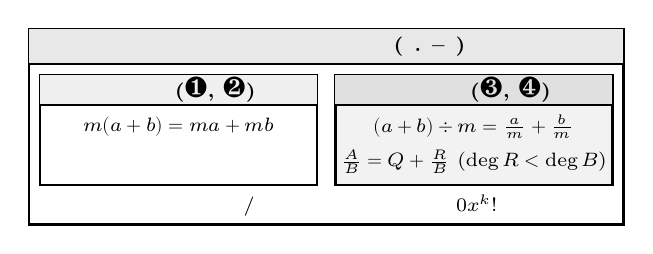
\begin{tikzpicture}[x=1cm, y=1cm, every node/.style={font=\scriptsize, text=black}]
  \draw[black, line width=0.9pt] (0,0) rectangle (7.55,2.48);
  \fill[gray!18] (0,2.04) rectangle (7.55,2.48);
  \draw[black, line width=0.6pt] (0,2.04) -- (7.55,2.04);
  \node at (3.775,2.26) {\textbf{សង្ខេបក្បួនគុណពហុធា និងក្បួនចែកពហុធា (ទំ.៦០--៦១)}};

  % Left: Multiplication
  \draw[black, line width=0.8pt] (0.14,0.50) rectangle (3.66,1.90);
  \fill[gray!12] (0.14,1.52) rectangle (3.66,1.90);
  \draw[black, line width=0.55pt] (0.14,1.52) -- (3.66,1.52);
  \node at (1.90,1.71) {\textbf{វិធីគុណពហុធា (\cnum{1}, \cnum{2})}};
  \node at (1.90,1.24) {$m(a+b) = ma + mb$};
  \node at (1.90,0.80) {គុណគ្រប់គូតួ រួចបង្រួម};

  % Right: Division
  \draw[black, line width=0.95pt, fill=gray!10] (3.89,0.50) rectangle (7.41,1.90);
  \fill[gray!24] (3.89,1.52) rectangle (7.41,1.90);
  \draw[black, line width=0.6pt] (3.89,1.52) -- (7.41,1.52);
  \node at (5.65,1.71) {\textbf{វិធីចែកពហុធា (\cnum{3}, \cnum{4})}};
  \node at (5.65,1.24) {$(a+b)\div m = \tfrac{a}{m} + \tfrac{b}{m}$};
  \node at (5.65,0.80) {$\tfrac{A}{B} = Q + \tfrac{R}{B}$ ($\deg R < \deg B$)};

  \node at (3.775,0.24) {\textbf{ប្រយ័ត្ន៖} មុនគុណ/ចែកជួរឈរ ត្រូវរៀបដឺក្រេចុះ និងថែមតួ $0x^k$!};
\end{tikzpicture}}

% ៤. E4 Elaborate: គុណជួរឈរ និងចែកពហុធាបាត់ខ្ទង់ (x^3 - 2)/(x - 1) (ទំ.៦០--៦២)
\newcommand{\figElaborateALGFiveFour}{%
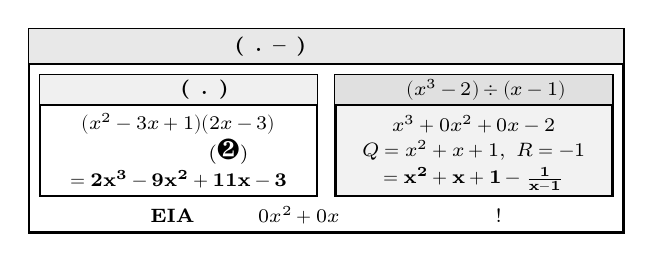
\begin{tikzpicture}[x=1cm, y=1cm, every node/.style={font=\scriptsize, text=black}]
  \draw[black, line width=0.9pt] (0,0) rectangle (7.55,2.58);
  \fill[gray!18] (0,2.14) rectangle (7.55,2.58);
  \draw[black, line width=0.6pt] (0,2.14) -- (7.55,2.14);
  \node at (3.775,2.36) {\textbf{លំហាត់គំរូ (ទំ.៦០--៦២)៖ គុណជួរឈរ និងចែកពហុធាបាត់ខ្ទង់}};

  % Left: (x^2 - 3x + 1)(2x - 3)
  \draw[black, line width=0.8pt] (0.14,0.46) rectangle (3.66,2.00);
  \fill[gray!12] (0.14,1.62) rectangle (3.66,2.00);
  \draw[black, line width=0.55pt] (0.14,1.62) -- (3.66,1.62);
  \node at (1.90,1.81) {\textbf{គុណជួរឈរ (ទំ.៦០)}};
  \node at (1.90,1.38) {$(x^2 - 3x + 1)(2x - 3)$};
  \node at (1.90,1.02) {រៀបដឺក្រេចុះជាមុន (\cnum{2})};
  \node at (1.90,0.68) {$= \mathbf{2x^3 - 9x^2 + 11x - 3}$};

  % Right: (x^3 - 2) / (x - 1)
  \draw[black, line width=0.95pt, fill=gray!10] (3.89,0.46) rectangle (7.41,2.00);
  \fill[gray!24] (3.89,1.62) rectangle (7.41,2.00);
  \draw[black, line width=0.6pt] (3.89,1.62) -- (7.41,1.62);
  \node at (5.65,1.81) {\textbf{ចែក $(x^3 - 2)\div(x - 1)$}};
  \node at (5.65,1.38) {$x^3 + 0x^2 + 0x - 2$};
  \node at (5.65,1.04) {$Q = x^2 + x + 1, \ R = -1$};
  \node at (5.65,0.68) {$= \mathbf{x^2 + x + 1 - \tfrac{1}{x-1}}$};

  \node at (3.775,0.22) {\textbf{\en{EIA}៖} បើមិនថែម $0x^2 + 0x$ ទេ នឹងដកខុសខ្ទង់ដឺក្រេភ្លាម!};
\end{tikzpicture}}

% ៥. E5 Evaluate: ជម្រើសវិនិច្ឆ័យ A-D គណនា (12x^3 - 6x) / (6x)
\newcommand{\figExitALGFiveFour}{%
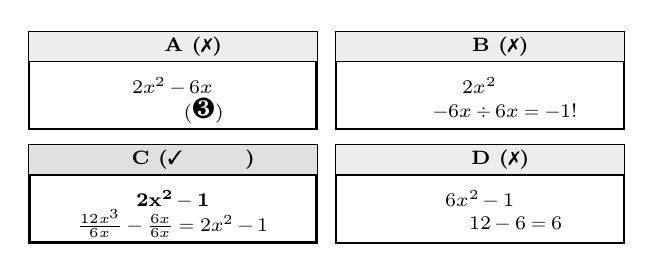
\begin{tikzpicture}[x=1cm, y=1cm, every node/.style={font=\scriptsize, text=black}]
  % Choice A
  \draw[black, line width=0.8pt] (0,1.44) rectangle (3.65,2.68);
  \fill[gray!14] (0,2.30) rectangle (3.65,2.68);
  \draw[black, line width=0.5pt] (0,2.30) -- (3.65,2.30);
  \node at (1.825,2.49) {\textbf{ជម្រើស \en{A} (\ding{55})}};
  \node at (1.825,2.00) {$2x^2 - 6x$};
  \node at (1.825,1.68) {ចែកតែតួទី១ (\cnum{3})};

  % Choice B
  \draw[black, line width=0.8pt] (3.90,1.44) rectangle (7.55,2.68);
  \fill[gray!14] (3.90,2.30) rectangle (7.55,2.68);
  \draw[black, line width=0.5pt] (3.90,2.30) -- (7.55,2.30);
  \node at (5.725,2.49) {\textbf{ជម្រើស \en{B} (\ding{55})}};
  \node at (5.725,2.00) {$2x^2$};
  \node at (5.725,1.68) {បំបាត់តួ $-6x \div 6x = -1$!};

  % Choice C (Correct)
  \draw[black, line width=1.05pt] (0,0) rectangle (3.65,1.24);
  \fill[gray!24] (0,0.86) rectangle (3.65,1.24);
  \draw[black, line width=0.6pt] (0,0.86) -- (3.65,0.86);
  \node at (1.825,1.05) {\textbf{ជម្រើស \en{C} (\ding{51} ត្រឹមត្រូវ)}};
  \node at (1.825,0.56) {$\mathbf{2x^2 - 1}$};
  \node at (1.825,0.24) {$\tfrac{12x^3}{6x} - \tfrac{6x}{6x} = 2x^2 - 1$};

  % Choice D
  \draw[black, line width=0.8pt] (3.90,0) rectangle (7.55,1.24);
  \fill[gray!14] (3.90,0.86) rectangle (7.55,1.24);
  \draw[black, line width=0.5pt] (3.90,0.86) -- (7.55,0.86);
  \node at (5.725,1.05) {\textbf{ជម្រើស \en{D} (\ding{55})}};
  \node at (5.725,0.56) {$6x^2 - 1$};
  \node at (5.725,0.24) {ច្រឡំដកមេគុណ $12 - 6 = 6$};
\end{tikzpicture}}

\begin{document}
\fontsize{10pt}{15.2pt}\selectfont

% ============================================================================
% ក្បាលរដ្ឋបាល (Administrative Header — តាមគំរូ ls_plan.tex)
% ============================================================================
{\centering
  {\muol\fontsize{11pt}{16pt}\selectfont ព្រះរាជាណាចក្រកម្ពុជា\par}
  {\muol\fontsize{11pt}{16pt}\selectfont ជាតិ សាសនា ព្រះមហាក្សត្រ\par}
  \vspace{-3pt}{\khmflourish\par}
}

\vspace{1pt}
{\muol\fontsize{10pt}{15.5pt}\selectfont
មន្ទីរអប់រំ យុវជន និងកីឡា ខេត្តកំពង់ធំ\par
ការិយាល័យអប់រំ យុវជន និងកីឡា ស្រុកកំពង់ស្វាយ\par
អនុវិទ្យាល័យព្រះក្រសាំង\par}

\vspace{2pt}
{\centering{\muol\fontsize{11.5pt}{17pt}\selectfont កិច្ចតែងការបង្រៀន\par}}
\vspace{2pt}

% --- ព័ត៌មានទូទៅ ---
{\hspace*{2.8cm}\renewcommand{\arraystretch}{1.08}
\begin{tabular}{@{}l@{\hspace{0.35cm}}p{2.9cm}@{\hspace{0.15cm}}c@{\hspace{0.25cm}}l@{}}
  - & មុខវិជ្ជា & : & គណិតវិទ្យា ថ្នាក់ទី៨ (ពីជគណិត) \\
  - & ចំណងជើងមេរៀន & : & មេរៀនទី៥៖ កន្សោមពីជគណិត \\
  - & ចំណងជើងរង & : & ២.៤ វិធីគុណពហុធា និង ២.៥ វិធីចែកពហុធា \\
  - & រយៈពេល & : & ១ ម៉ោងសិក្សា (៥០ នាទី) \\
  - & បង្រៀនដោយ & : & ហុក ប៊ុនថែន \\
  - & កាលបរិច្ឆេទ & : & ថ្ងៃអង្គារ ទី៨ ខែធ្នូ ឆ្នាំ២០២៦ \\
\end{tabular}\par}

\vspace{2pt}

% --- I. វត្ថុបំណង ---
{\muol\fontsize{10pt}{15.5pt}\selectfont \enbf{I.} វត្ថុបំណង\par}
\vspace{1pt}
{\renewcommand{\arraystretch}{1.10}
\begin{tabular}{@{}p{0.55cm}@{}p{2.35cm}@{\hspace{0.15cm}}c@{\hspace{0.25cm}}p{14.95cm}@{}}
  \hfill\wcirc\hspace{0.2cm} & វិជ្ជាសម្បទា & : & សិស្សប្រាប់ក្បួនគុណឯកធានឹងពហុធា គុណពហុធានឹងពហុធា ចែកពហុធានឹងឯកធា និងចែកពហុធានឹងពហុធាបានត្រឹមត្រូវ (ទំ.៥៩--៦២) ។ \\
  \hfill\wcirc\hspace{0.2cm} & បំណិនសម្បទា & : & សិស្សគណនាផលគុណនិងផលចែកពហុធាតាមជួរដេកនិងជួរឈរ (ដោយរៀបដឺក្រេចុះ និងថែមតួ $0x^k$ ពេលបាត់ខ្ទង់) លើសន្លឹកកិច្ចការបានត្រឹមត្រូវ ។ \\
  \hfill\wcirc\hspace{0.2cm} & ចរិយាសម្បទា & : & សិស្សមានទម្លាប់ប្រុងប្រយ័ត្នខ្ពស់ក្នុងការចែកគ្រប់តួទាំងអស់នៃពហុធា និងផ្ទៀងផ្ទាត់សំណល់តាមរូបមន្ត $A = B\cdot Q + R$ ។ \\
\end{tabular}\par}

\vspace{2pt}

% --- II. សម្ភារៈឧបទេស ---
{\muol\fontsize{10pt}{15.5pt}\selectfont \enbf{II.} សម្ភារៈឧបទេស\par}
\vspace{1pt}
\hspace*{0.55cm}$\bullet$\ សៀវភៅសិក្សាគោលថ្នាក់ទី៨ (ទំ.៥៩--៦២, ៧២--៧៣) ក្ដារខៀន ដីស/ហ្វឺត បន្ទាត់ត្រង់ និង\textbf{សន្លឹកកិច្ចការសិស្សបំពេញចន្លោះ ស-ខ្មៅ} (កូដ \en{ALG54} ទំព័រ ១--២ សម្រាប់សិស្ស និងទំព័រ ៣ ប្លង់ក្ដារខៀន/ចម្លើយគ្រូ — គ្មានប្រើ \en{LCD})\par

\vspace{2pt}

% --- III. វិធីសាស្រ្តបង្រៀន ---
{\muol\fontsize{10pt}{15.5pt}\selectfont \enbf{III.} វិធីសាស្រ្តបង្រៀន\par}
\vspace{1pt}
{\renewcommand{\arraystretch}{1.08}
\begin{tabular}{@{}p{0.55cm}@{}p{2.35cm}@{\hspace{0.15cm}}c@{\hspace{0.25cm}}p{14.95cm}@{}}
  \hfill$\bullet$\hspace{0.2cm} & គោលវិធី & : & សិស្សមជ្ឈមណ្ឌល (សន្លឹកកិច្ចការបំពេញចន្លោះជាគោល + ការពិភាក្សាជាក្រុមតូច ៣ នាក់) \\
  \hfill$\bullet$\hspace{0.2cm} & យុទ្ធវិធីបង្រៀន & : & គំរូស្ថាបនានិយម \en{5Es} រួមបញ្ចូល \textbf{គំរូផ្ទៃក្រឡាប្រអប់ (\en{Area Box Model})} និង \textbf{ការថែមខ្ទង់ $0x^k$ ក្នុងវិធីចែកពហុធាជួរឈរ} \\
\end{tabular}\par}

\vspace{2pt}

% --- IV. ដំណើរការបង្រៀន ---
{\muol\fontsize{10pt}{15.5pt}\selectfont \enbf{IV.} ដំណើរការបង្រៀន\par}

{\renewcommand{\arraystretch}{1.15}
\begin{longtable}{|L{5.50cm}|L{7.90cm}|L{4.80cm}|}
\hline
\multicolumn{1}{|c|}{\cellcolor{headgray}\muol សកម្មភាពគ្រូ} &
\multicolumn{1}{c|}{\cellcolor{headgray}\muol ខ្លឹមសារមេរៀន} &
\multicolumn{1}{c|}{\cellcolor{headgray}\muol សកម្មភាពសិស្ស} \\
\hline
\endfirsthead

\hline
\multicolumn{1}{|c|}{\cellcolor{headgray}\muol សកម្មភាពគ្រូ} &
\multicolumn{1}{c|}{\cellcolor{headgray}\muol ខ្លឹមសារមេរៀន} &
\multicolumn{1}{c|}{\cellcolor{headgray}\muol សកម្មភាពសិស្ស} \\
\hline
\endhead

% ==================== ជំហានទី១ (2min) ====================
\stepheader{ជំហានទី១ \enbf{(}រដ្ឋបាលថ្នាក់\enbf{)}}
$\bullet$ ពិនិត្យវត្តមាន អនាម័យ និងសណ្ដាប់ធ្នាប់ថ្នាក់រៀន \par
$\bullet$ រៀបចំក្រុមតូច ៣ នាក់ និងចែក\textbf{សន្លឹកកិច្ចការសិស្ស (\en{ALG54} ទំព័រ ១–២)}
&
$\bullet$ រដ្ឋបាលថ្នាក់ អនាម័យ និងវិន័យសិក្សា \par
$\bullet$ ចែកសន្លឹកកិច្ចការម្នាក់ ១ សន្លឹក សម្រាប់បំពេញតាមដំណាក់កាល \en{E1--E5}
&
$\circ$ ប្រធានថ្នាក់រាយការណ៍វត្តមានសិស្ស \par
$\circ$ ទទួលសន្លឹកកិច្ចការ សរសេរឈ្មោះ និងអង្គុយតាមក្រុម ៣ នាក់ \\
\hline

% ==================== ជំហានទី២ (9min: កំណែ <=3m + រំលឹក 3m + E1 3m) ====================
\stepheader{ជំហានទី២ \enbf{(}កិច្ចការផ្ទះ \enbf{+} ទំនាក់ទំនងមេរៀនថ្មី\enbf{)}}
\ditem \textbf{កំណែកិច្ចការផ្ទះ ($\le\text{\enbf{3\,min}}$)} \par
$\bullet$ ហៅសិស្ស ២ នាក់ឡើងកែលំហាត់ទំ.៥៩ (គ) និងទំ.៧២–៧៣ \#4, \#5 ខ លើក្ដារខៀន
&
{\centering\redsub{កំណែកិច្ចការផ្ទះ (ទំ.៥៩ គ និង ទំ.៧២–៧៣ \#4, \#5 ខ)}\par}
$\bullet$ \textbf{ទំ.៥៩ (គ)៖} $M+N = \mathbf{2xy^2-10xy-19}$; \ $M-N = \mathbf{-xy^2+14xy+13}$ \par
$\bullet$ \textbf{\#4៖} $A-B = \mathbf{3x^4+3x^3+x^2-2x-2}$; \ \textbf{\#5 ខ៖} $\mathbf{7a^3b^2-4ab}$
&
$\circ$ ផ្ទៀងចម្លើយ និងកែតម្រូវចូលសៀវភៅកិច្ចការផ្ទះ \\[3pt]

\ditem \textbf{រំលឹកមេរៀនទាក់ទង (\enbf{3min})} \par
$\bullet$ សួរ៖ «តើ $3x^2 \cdot 4x^3$ និង $(-30x^6)\div(5x^2)$ ស្មើប៉ុន្មាន? ចុះលក្ខណៈបំបែក $m(a+b)$ ស្មើអ្វី?»
&
{\centering\redsub{រំលឹកគុណ/ចែកឯកធា និងលក្ខណៈបំបែក}\par}
$\bullet$ $3x^2 \cdot 4x^3 = \mathbf{12x^5}$ \quad និង \quad $(-30x^6)\div(5x^2) = \mathbf{-6x^4}$ \par
$\bullet$ លក្ខណៈបំបែក៖ $m(a + b) = ma + mb$
&
$\circ$ ឆ្លើយ៖ «$12x^5$; $-6x^4$; និង $ma + mb$!» \\[3pt]

\fiveE{E1 - Engage (3min)} \timenote{(កុំទាន់ផ្ដល់ចម្លើយ)} \par
\ditem \textbf{បេសកកម្មអន្ទាក់សម្រួលតែតួទី១ (សន្លឹកកិច្ចការ \en{E1})} \par
$\bullet$ ឱ្យសិស្សអានប្រអប់ \en{E1} ហើយគូសជ្រើសរើសរវាង\textbf{សិស្ស ក} និង\textbf{សិស្ស ខ}
&
\redsub{បេសកកម្ម \en{E1}៖ គណនាផលចែក $(15x^4 - 30x^6) \div (5x^2)$ (ទំ.៦០)} \par
$\bullet$ \textbf{សិស្ស ក} សម្រួលតែតួទី១ $\tfrac{15x^4 - 30x^6}{5x^2}$ បាន $3x^2 - 30x^6$! \par
$\bullet$ \textbf{សិស្ស ខ} ចែកគ្រប់តួទាំងពីរនឹង $5x^2$ បាន $3x^2 - 6x^4$! តើអ្នកណាត្រូវ?
&
$\circ$ ពិភាក្សាជាគូ និងគូស \ding{51} ក្នុងប្រអប់ \en{E1} លើសន្លឹកកិច្ចការ \\[3pt]

&
\cfig{\figEngageALGFiveFour}
& \\
\hline

% ==================== ជំហានទី៣ (17min: E2 11m + E3 6m) ====================
\stepheader{ជំហានទី៣ \enbf{(}ខ្លឹមសារមេរៀនថ្មី\enbf{)}}
\fiveE{E2 - Explore (11min)} \par
$\bullet$ សរសេរចំណងជើងរង \textbf{២.៤ វិធីគុណពហុធា និង ២.៥ វិធីចែកពហុធា} លើក្ដារខៀន \par
\ditem \textbf{សកម្មភាព ១៖ វិធីគុណពហុធា (ទំ.៥៩–៦០, \enbf{5min}, \en{E2-A})} \par
$\bullet$ ឱ្យសិស្សគណនាផ្ទៃរូបថតប្រាសាទ $(3x+2)(x+1)$ និងគំរូទី ១ លើ \en{E2-A}
&
២.៤ វិធីគុណពហុធា (ទំ.៥៩–៦០) \par
$\bullet$ \textbf{គុណឯកធានឹងពហុធា៖} $x(3x+1) = 3x^2+x$; \ $3x^2(4x^3+xy-5y^2) = \mathbf{12x^5+3x^3y-15x^2y^2}$ \par
$\bullet$ \textbf{គុណពហុធានឹងពហុធា (រូបថតប្រាសាទ ទំ.៥៩)៖} $(3x+2)(x+1) = 3x(x+1)+2(x+1) = 3x^2+3x+2x+2 = \mathbf{3x^2+5x+2}$
&
$\circ$ បំពេញក្រឡាផ្ទៃក្រឡា និងពន្លាតផលគុណពហុធាលើ \en{E2-A} \\[3pt]

\ditem \textbf{សកម្មភាព ២៖ វិធីចែកពហុធា (ទំ.៦០–៦១, \enbf{6min}, \en{E2-B})} \par
$\bullet$ ឱ្យសិស្សគណនាផលចែកពហុធានឹងឯកធា និងចែកជួរឈរឧទាហរណ៍ ៣–៤ លើ \en{E2-B}
&
២.៥ វិធីចែកពហុធា (ទំ.៦០–៦១) \par
$\bullet$ \textbf{ចែកពហុធានឹងឯកធា៖} $(6x^3+8x^2+10x)\div(2x) = \mathbf{3x^2+4x+5}$ \par
$\bullet$ \textbf{ចែកពហុធានឹងពហុធា (ទំ.៦១)៖} $(x^2-7x+10)\div(x-2) = \mathbf{x-5}$ (សំណល់ $0$, ចែកដាច់); \quad $(x^2-2x+4)\div(x-1) = \mathbf{x-1 + \tfrac{3}{x-1}}$
&
$\circ$ គណនាផលចែកពហុធានឹងឯកធា និងចែកជួរឈរលើ \en{E2-B} \\[3pt]

&
\cfig{\figExploreALGFiveFour}
& \\[3pt]

% --- E3 Explain (6min) ---
\fiveE{E3 - Explain (6min)} \par
$\bullet$ ដឹកនាំសិស្សសង្ខេបក្បួនគុណពហុធា និងក្បួនចែកពហុធា (ទំ.៦០–៦១)
&
$\bullet$ \textbf{ក្បួនគុណ និងចែកពហុធា (ទំ.៦០–៦១)៖} \par
\hspace*{0.15cm}១) \textbf{គុណពហុធា៖} គុណតួនីមួយៗនៃពហុធាទី១ នឹងគ្រប់តួនៃពហុធាទី២ រួច\graybox{បង្រួមឯកធាដូចគ្នា} \par
\hspace*{0.15cm}២) \textbf{ចែកពហុធានឹងឯកធា៖} ចែក\textbf{គ្រប់តួទាំងអស់}នៃពហុធានឹងឯកធានោះ រួចបូកលទ្ធផល \par
\hspace*{0.15cm}៣) \textbf{ចែកពហុធា $A$ នឹង $B$៖} $\dfrac{A}{B} = Q + \dfrac{R}{B}$ (បើសំណល់ $R = 0$ នោះ $A$ ចែកដាច់នឹង $B$)
&
$\circ$ បំពេញប្រអប់ក្បួនគោលទាំង ៣ លើសន្លឹកកិច្ចការ \en{E3} \\[3pt]

$\bullet$ ភ្ជាប់\textbf{ធនាគារហេតុផល \cnum{1}--\cnum{4}} លើក្ដារខៀន និងសន្លឹកកិច្ចការ
&
\textbf{ធនាគារហេតុផល (\en{Warrant Bank})៖} \par
\cnum{1} \textbf{គុណបំបែក៖} គុណគ្រប់គូតួទាំងអស់ ដោយប្រយ័ត្នសញ្ញាផលគុណ ($-\times - = +$) \par
\cnum{2} \textbf{រៀបដឺក្រេចុះ៖} មុនគុណ ឬចែកតាមជួរឈរ ត្រូវរៀបពហុធាតាមដឺក្រេចុះជាមុន
&
$\circ$ ផ្ទៀងលេខកូដ \cnum{1}--\cnum{2} លើសន្លឹកកិច្ចការ \\[3pt]

&
\cnum{3} \textbf{ចែកគ្រប់តួ៖} ហាមសម្រួលតែតួទី១ ហើយបើតួចែកនឹងខ្លួនឯងត្រូវនៅសល់ $\pm 1$ \par
\cnum{4} \textbf{ថែមខ្ទង់ $0x^k$៖} ពេលចែកពហុធាបាត់ខ្ទង់ ត្រូវសរសេរ $0x^k$ ដើម្បីកុំឱ្យដកខុសខ្ទង់
&
$\circ$ ផ្ទៀងលេខកូដ \cnum{3}--\cnum{4} លើសន្លឹកកិច្ចការ \\[3pt]

&
\cfig{\figRuleALGFiveFour}
& \\
\hline

% ==================== ជំហានទី៤ (20min: E4 10m + E5 10m) ====================
\stepheader{ជំហានទី៤ \enbf{(}ពង្រីកចំណេះដឹង\enbf{)}}
\fiveE{E4 - Elaborate (10min)} \par
\ditem \textbf{លំហាត់គំរូ៖ គុណជួរឈរ និងចែកពហុធាបាត់ខ្ទង់ (ទំ.៦០–៦២)} \par
$\bullet$ ឱ្យសិស្សធ្វើលំហាត់គំរូទី ២–៣ (ទំ.៦០) និងគំរូទី ១–២ (ទំ.៦១–៦២) លើ \en{E4}
&
{\muol លំហាត់គំរូ} \textbf{(ទំ.៦០–៦២)៖} \par
$\bullet$ \textbf{១) គុណជួរឈរ និងពហុធាគោល ១០ (ទំ.៦០)៖} \par
\hspace*{0.2cm}-- $(1+x^2-3x)(2x-3) = (x^2-3x+1)(2x-3) = \graybox{$2x^3 - 9x^2 + 11x - 3$}$ \par
\hspace*{0.2cm}-- $7\,368 = 7\times 10^3 + 3\times 10^2 + 6\times 10 + 8$ \par
$\bullet$ \textbf{២) ចែកពហុធាបាត់ខ្ទង់ (ទំ.៦១–៦២)៖} \par
\hspace*{0.2cm}-- $(8y^3+4y^2+0y-7)\div(2y+3) = \mathbf{4y^2 - 4y + 6 - \tfrac{25}{2y+3}}$ \par
\hspace*{0.2cm}-- $(x^3+0x^2+0x-2)\div(x-1) = \graybox{$x^2 + x + 1 - \tfrac{1}{x-1}$}$ \par
\hspace*{0.2cm}-- \textbf{ផ្ទៀងផ្ទាត់៖} $(x-1)(x^2+x+1) + (-1) = (x^3-1)-1 = x^3-2$ (\ding{51})
&
$\circ$ រៀបដឺក្រេចុះ ថែមខ្ទង់ $0y, 0x^2, 0x$ និងគណនាផលគុណ/ផលចែកត្រឹមត្រូវ \\[3pt]

&
\cfig{\figElaborateALGFiveFour}
& \\[3pt]

$\bullet$ សួរសំណួរឆ្លុះបញ្ចាំង \textbf{\en{EIA Looking-Back} (1min)}
&
\textbf{\en{EIA Looking-Back}៖} «ពេលចែក $(a^2b^3 + 2ab)\div(ab)$ (ទំ.៦២ ក) ហេតុអ្វីចម្លើយស្មើ $ab^2 + 2$ មិនមែនស្មើ $ab^2$ ទទេ?» ($\to$ ព្រោះតួទី២ គឺ $\tfrac{2ab}{ab} = 2\times 1 = 2$ មិនមែនសូន្យទេ!)
&
$\circ$ ពន្យល់ថា $\tfrac{2ab}{ab} = 2$ ត្រូវរក្សាទុកជានិច្ច (\cnum{3}) \\[3pt]

% --- E5 Evaluate (10min) ---
\fiveE{E5 - Evaluate (10min)} \par
\ditem \textbf{ប្រតិបត្តិជាក្រុមតូច ៣ នាក់ (4min, សន្លឹកកិច្ចការ \en{E5})} \par
$\bullet$ ឱ្យសិស្សដោះស្រាយប្រតិបត្តិទំ.៦០ (ក) និងទំ.៦២ (ក, គ)
&
{\muol លំហាត់ប្រតិបត្តិ} \textbf{(ទំ.៦០ និង ទំ.៦២)៖} \par
$\bullet$ \textbf{១) ទំ.៦០ (ក)៖} $2x^2(2x^2+3x-1) = \mathbf{4x^4 + 6x^3 - 2x^2}$ \par
$\bullet$ \textbf{២) ទំ.៦២ (ក) និង (គ)៖} $(a^2b^3+2ab)\div(ab) = \mathbf{ab^2 + 2}$; \quad $(6x^2+5x-4)\div(2x-1) = \mathbf{3x + 4}$ (សំណល់ $0$)
&
$\circ$ គណនាជាក្រុមឃើញ $4x^4+6x^3-2x^2, ab^2+2$ និង $3x+4$ \\[3pt]

$\bullet$ ឱ្យក្រុមសិស្សផ្ទៀងផ្ទាត់និង\textbf{បិទបេសកកម្ម \en{E1} (2min)}
&
$\bullet$ \textbf{បិទបេសកកម្ម \en{E1}៖} សិស្ស ខ ត្រឹមត្រូវ! $(15x^4-30x^6)\div(5x^2) = \tfrac{15x^4}{5x^2} - \tfrac{30x^6}{5x^2} = \mathbf{3x^2 - 6x^4}$!
&
$\circ$ បិទបេសកកម្ម \en{E1} ឃើញសិស្ស ខ ត្រឹមត្រូវ \\[3pt]

\ditem \textbf{សំណួរវិនិច្ឆ័យ \en{A--D} និងសំបុត្រចេញ (4min)} \par
$\bullet$ ឱ្យសិស្សគូសរង្វង់ជម្រើសត្រូវលើសន្លឹកកិច្ចការ រួចលើកម្រាមដៃ ១--៤
&
{\centering\textbf{សំណួរវិនិច្ឆ័យ \en{A--D}៖ គណនាផលចែក $(12x^3 - 6x) \div (6x)$}\par}
{\centering \enbf{A.}\ $2x^2 - 6x$ \quad \enbf{B.}\ $2x^2$ \quad \enbf{C.}\ $2x^2 - 1$ \quad \enbf{D.}\ $6x^2 - 1$\par}
{\centering\textit{(កត់សម្គាល់៖ ចែកគ្រប់តួទាំងពីរ ហើយប្រយ័ត្នតួ $-6x \div 6x$)}\par}
&
$\circ$ គណនា និងលើកម្រាមដៃ ៣ (\textbf{ជម្រើស \en{C}៖ $2x^2 - 1$}) \\[3pt]

&
\cfig{\figExitALGFiveFour}
& \\[3pt]

$\bullet$ បញ្ជាក់ចម្លើយត្រូវ (\textbf{ជម្រើស \en{C}}) និងឱ្យបំពេញ\textbf{សំបុត្រចេញ ៦០ វិនាទី}
&
$\bullet$ \textbf{សំបុត្រចេញ៖} ពន្លាតផលគុណ $(x + 2)(x - 5) = x^2 - 5x + 2x - 10 = \mathbf{x^2 - 3x - 10}$ ។
&
$\circ$ បំពេញសំបុត្រចេញលើសន្លឹកកិច្ចការមុនបញ្ចប់ម៉ោង \\
\hline

% ==================== ជំហានទី៥ (<=2min) ====================
\stepheader{ជំហានទី៥ \enbf{(}កិច្ចការផ្ទះ \enbf{+} បណ្ដាំផ្ញើ\enbf{)}}
\timenote{ចំណាយពេលឱ្យតិចបំផុតកុំឱ្យលើស 2min} \par
$\bullet$ ណែនាំប្រអប់\textbf{កិច្ចការផ្ទះ}លើសន្លឹកកិច្ចការទំព័រ ២ (ទំ.៦០, ៦២ និងទំ.៧២–៧៣ \#2, \#6)
&
{\centering{\muol កិច្ចការផ្ទះ} \textbf{(សៀវភៅគោល ទំ.៦០, ៦២ និង ទំ.៧២–៧៣ \#2, \#6)}\par} \par
$\bullet$ \textbf{១) ប្រតិបត្តិទំ.៦០ (គ, ង) និង ទំ.៦២ (ខ, ឃ)៖} គណនា $(a^2+2ab)(a-b)$, $\tfrac{1}{2}xy^2(\tfrac{2}{3}xy-3)$, $(5x^2y^4+2x^3y^5-12x^2y^2)\div(x^2y^2)$ និង $(a^2+6a-55)\div(a-5)$ ។ \par
$\bullet$ \textbf{២) លំហាត់ \#2 (ទំ.៧២) និង \#6 (ទំ.៧៣)៖} សរសេរ $1997, 2674$ ជាពហុធាដឺក្រេចុះនៃ $10$; និងបង្រួម $a(x-b)-b(a-x)+x(a+b)$ ។
&
$\circ$ គូសចំណាំកិច្ចការផ្ទះលើសន្លឹកកិច្ចការ \\[3pt]

$\bullet$ ផ្ដាំផ្ញើឱ្យអានមុនចំណុច ៣.១ (សមភាពសំខាន់ៗ៖ ការេនៃទ្វេធា និងផលគុណផលបូកនិងផលដក)
&
$\bullet$ \textbf{បណ្ដាំផ្ញើ៖} អានមុន \textbf{៣.១ ពន្លាតការេនៃទ្វេធា និង $(a-b)(a+b)$ (ទំ.៦៣–៦៦)} ។
&
$\circ$ កត់ត្រាបណ្ដាំផ្ញើ ទុកសន្លឹកកិច្ចការក្នុងសៀវភៅ និងជម្រាបលាគ្រូ \\
\hline
\end{longtable}}

\vspace{6pt}
% --- ហត្ថលេខា (កាលបរិច្ឆេទត្រូវគ្នា ១០០% នឹងខាងលើ) ---
{\centering
\hspace*{5.2cm}\begin{minipage}{11.5cm}
  \centering
  ថ្ងៃអង្គារ ១៤រោច ខែកត្តិក ឆ្នាំមមី អដ្ឋស័ក ពុទ្ធសករាជ ២៥៧០\par
  កំពង់ស្វាយ, ថ្ងៃទី៨ ខែធ្នូ ឆ្នាំ២០២៦\par
  \vspace{2pt}
  {\muol គ្រូបង្រៀន\par}
  \vspace{32pt}
  \hfill{\muol ហុក ប៊ុនថែន}\hspace*{1.4cm}
\end{minipage}\par}

\end{document}
